% !TEX TS-program = xelatex
% !TEX encoding = UTF-8 Unicode
% !Mode:: "TeX:UTF-8"

\documentclass{resume}
\usepackage{zh_CN-Adobefonts_external} % Simplified Chinese Support using external fonts (./fonts/zh_CN-Adobe/)
%\usepackage{zh_CN-Adobefonts_internal} % Simplified Chinese Support using system fonts
\usepackage{linespacing_fix} % disable extra space before next section
\usepackage{cite}
\usepackage{multirow}

\usepackage{fontmfizz}

\usepackage{geometry}
\geometry{a4paper,left=1cm,right=1cm,top=0.5cm,bottom=0.5cm}

\begin{document}

\pagenumbering{gobble} % suppress displaying page number





%%%%%%%%%%%%%%%%%%%%%%%%%%%%%%%%%%%%%%%%%%%%%%%%%%%%%%%%%%%%%%%%%%%%%%%%%%%%%%%%%%%%%%%%%%%%%%%%%%%%%%%%%%%%%%%%%%%%%%%%%%%%%%%%%%%%%%%%%%%%%%%%%%%%%%%%%%
%
%
%                                                                 简介
%
%
%%%%%%%%%%%%%%%%%%%%%%%%%%%%%%%%%%%%%%%%%%%%%%%%%%%%%%%%%%%%%%%%%%%%%%%%%%%%%%%%%%%%%%%%%%%%%%%%%%%%%%%%%%%%%%%%%%%%%%%%%%%%%%%%%%%%%%%%%%%%%%%%%%%%%%%%%%%








\name{\quad\quad\quad \quad\quad\quad\quad\quad \\ 徐玉全 \\ \\ \quad \quad\quad
 \multirow{4}{0.6in}{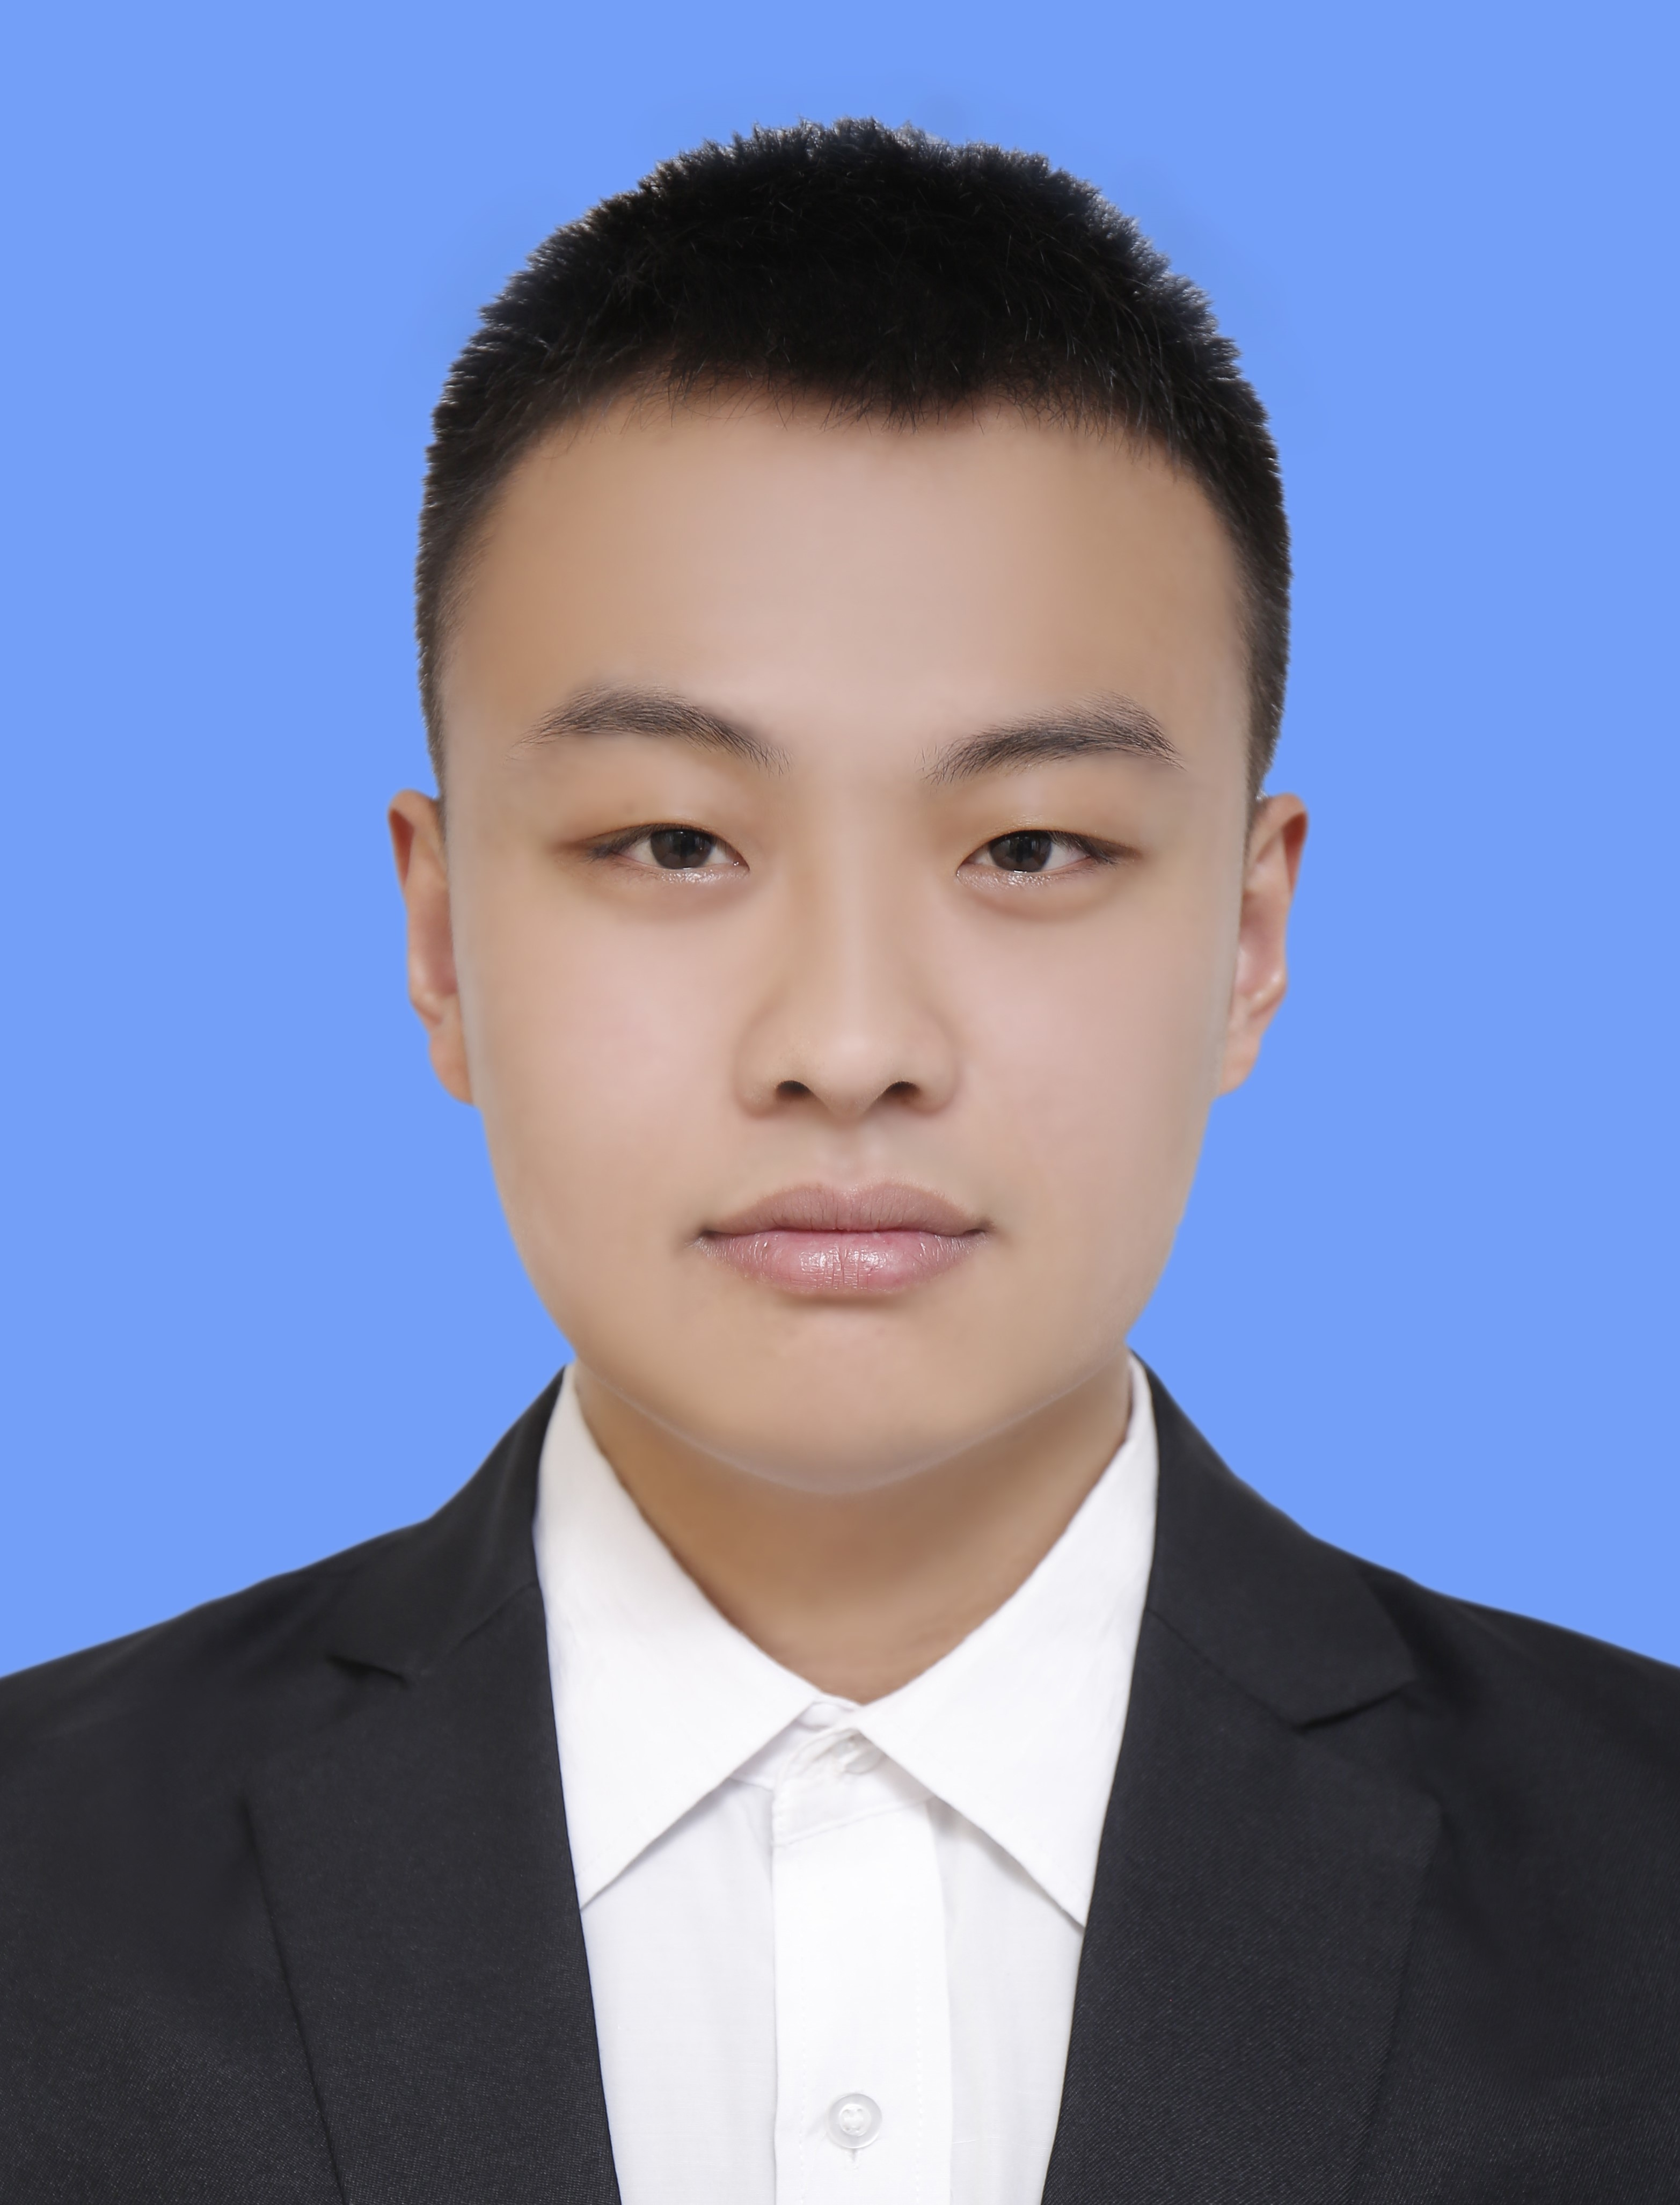
\includegraphics[width=1.1 in]{qq}}} 


\quad \\ \quad

\basicInfo{

\email{xuyuquan713@163.com} \textperiodcentered\
  \phone{(+86) 166-0561-0713} \textperiodcentered\
  \linkedin [安徽 淮北]{https://xuyuquan0713.github.io/} 
}


\quad\quad\quad\quad \quad\quad\quad\quad\quad \faFire\quad \faLink {www.zhiyuquan.top}  \quad \quad \textperiodcentered\ \faEnvira \quad\textbf {控制工程}  \quad\quad\quad \quad \quad\quad \textperiodcentered\  \faFire  \textbf{硕 士}
\\  
\\


\datedsubsection{ \textbf{\Large { 应聘岗位:嵌入式软件工程师}}}{}

%%%%%%%%%%%%%%%%%%%%%%%%%%%%%%%%%%%%%%%%%%%%%%%%%%%%%%%%%%%%%%%%%%%%%%%%%%%%%%%%%%%%%%%%%%%%%%%%%%%%%%%%%%%%%%%%%%%%%%%%%%%%%%%%%%%%%%%%%%%%%%%%%%%%%%%%%%
%
%
%                                                                 教育背景
%
%
%%%%%%%%%%%%%%%%%%%%%%%%%%%%%%%%%%%%%%%%%%%%%%%%%%%%%%%%%%%%%%%%%%%%%%%%%%%%%%%%%%%%%%%%%%%%%%%%%%%%%%%%%%%%%%%%%%%%%%%%%%%%%%%%%%%%%%%%%%%%%%%%%%%%%%%%%%%




\section{\faGraduationCap\  教育背景}
\datedsubsection{\textbf{合肥工业大学},\quad  合肥}{2019 -- 至今}
\textit{研究生}\ \quad \quad 控制工程  \\ \textit{研究方向} \quad 机器人
\datedsubsection{\textbf{长春大学},\quad  长春}{2015 -- 2019}
\textit{本科}\  \quad \quad\quad 自动化
\datedsubsection{\textbf{中国人民解放军},\quad  陆军}{2013 -- 2015}
\textit{参军入伍}\








%%%%%%%%%%%%%%%%%%%%%%%%%%%%%%%%%%%%%%%%%%%%%%%%%%%%%%%%%%%%%%%%%%%%%%%%%%%%%%%%%%%%%%%%%%%%%%%%%%%%%%%%%%%%%%%%%%%%%%%%%%%%%%%%%%%%%%%%%%%%%%%%%%%%%%%%%%
%
%
%                                                                 技能
%
%
%%%%%%%%%%%%%%%%%%%%%%%%%%%%%%%%%%%%%%%%%%%%%%%%%%%%%%%%%%%%%%%%%%%%%%%%%%%%%%%%%%%%%%%%%%%%%%%%%%%%%%%%%%%%%%%%%%%%%%%%%%%%%%%%%%%%%%%%%%%%%%%%%%%%%%%%%%%




\section{\faCogs\  技能}
% increase linespacing [parsep=0.5ex]
\begin{itemize}[parsep=0.5ex]
  \item 编程语言: 熟练使用C/C++,Matlab,Makefile,了解Python,shell/bash语言编程,熟悉TCP/IP网络编程
  \item 平台: 熟悉Linux,Windows开发环境,有Linux环境开发经验,了解 RT-Thread操作系统
   \item 硬件开发工具:熟练使用AltiunDesigner、KiCad原理图和PCB绘制软件
  \item 软件开发工具: 熟练使用\faGit 版本开发工具,gdb,keil,Code Composer Studio,STM32cubeMX嵌入式开发工具
  \item 英语能力:英语四级,能够流畅阅读外文文献
  \item 排版工具:Markdown,\LaTeX,计算机二级(C语言)
\end{itemize}







%%%%%%%%%%%%%%%%%%%%%%%%%%%%%%%%%%%%%%%%%%%%%%%%%%%%%%%%%%%%%%%%%%%%%%%%%%%%%%%%%%%%%%%%%%%%%%%%%%%%%%%%%%%%%%%%%%%%%%%%%%%%%%%%%%%%%%%%%%%%%%%%%%%%%%%%%%
%
%
%                                                                 实习/项目经历
%
%
%%%%%%%%%%%%%%%%%%%%%%%%%%%%%%%%%%%%%%%%%%%%%%%%%%%%%%%%%%%%%%%%%%%%%%%%%%%%%%%%%%%%%%%%%%%%%%%%%%%%%%%%%%%%%%%%%%%%%%%%%%%%%%%%%%%%%%%%%%%%%%%%%%%%%%%%%%%









\section{\faUsers\ 项目经历}


\datedsubsection{\textbf{狭窄空间下的路径规划算法研究}\quad \quad \quad  \quad 安徽省重大课题专项}{2020年9月 -- 至今}
\role{项目描述}{}            %%%安徽省重大课题专项:复杂场景下的智能柔性探伤机器人关键技术
\begin{onehalfspacing}
  为了解决一些在狭窄空间下路径规划困难的问题,对狭窄空间下的路径规划方法进行研究。\\
  \textbf {主要工作:}
  \begin{itemize}

    \item 针对狭窄空间路径规划问题和发展现状进行调研,总结路径规划的问题和解决办法。
    \item 针对基于采样算法在多维空间下采样问题对算法进行优化和仿真实验,提出改进算法。%改进的算法可以很好的解决在狭窄空间下的路径规划实时性差和准确度低的问题。
    \item 对仿真的实验数据使用Python和Matlab进行数据处理。
   %% \item 针对改进的算法使用Vrep建模同时使用python进行联合仿真。
    \item 书写小论文。
  \end{itemize}

\end{onehalfspacing}

\datedsubsection{\textbf{ 基于MSP432平台的机器人迷宫路径规划算法编写}}{2019 年9月 -- 2019年12月}
%%\role{ 基于MSP432平台的机器人迷宫路径规划算法编写}{实验室项目}
\role{项目描述}{}
\begin{onehalfspacing}
  实验室和TI公司合作开发迷宫机器人套件。该套件以MSP432单片机为核心,根据单片机的片上资源设计各类电路,包括电源模块、电机驱动模块、陀螺仪模块、超声波测距模块、红外传感器模块、显示模块等。\\  
  \textbf {主要工作:}
  \begin{itemize}

    \item 编写迷宫核心算法并进行算法优化。
    \item 调试Pid算法控制迷宫机器人。
     \item 使用模糊Pid算法控制迷宫机器人。
    \item 绘制电路原理图和PCB,制版焊接调试。
    \item 基于迷宫机器人套件编写相应的技术文档。
  \end{itemize}
\end{onehalfspacing}






%%                                                   自己编写的破项目

\datedsubsection{\textbf{ 基于Mini2440开发板的移动机器人程序编写}}{2020 年3月 -- 2020年8月}

\role{项目描述}{}
\begin{onehalfspacing}
  基于实验室Mini开发板学习套件,该套件以Samsung S3c2440A芯片为核心。\\
   \textbf {开发环境/工具:}  Linux环境,arm-linux-gcc,Vim,Makefile\\
  \textbf {主要工作:}
  \begin{itemize}

    \item 内核的编译和移植,内核下载和NFS文件系统的搭建。
    \item 移植madplay,使用交叉编译器编译madplay,烧写下载madplay并编写脚本播放mp3音乐。
    \item 应用层程序编写,实现循迹、倒车雷达、温度检测、报警等功能。
    \item 文档整理,编写使用手册。
  \end{itemize}

\end{onehalfspacing}


% Reference Test
%\datedsubsection{\textbf{Paper Title\cite{zaharia2012resilient}}}{May. 2015}
%An xxx optimized for xxx\cite{verma2015large}
%\begin{itemize}
%  \item main contribution
%\end{itemize}


%%%%%%%%%%%%%%%%%%%%%%%%%%%%%%%%%%%%%%%%%%%%%%%%%%%%%%%%%%%%%%%%%%%%%%%%%%%%%%%%%%%%%%%%%%%%%%%%%%%%%%%%%%%%%%%%%%%%%%%%%%%%%%%%%%%%%%%%%%%%%%%%%%%%%%%%%%
%
%
%                                                                 个人开源项目情况
%
%
%%%%%%%%%%%%%%%%%%%%%%%%%%%%%%%%%%%%%%%%%%%%%%%%%%%%%%%%%%%%%%%%%%%%%%%%%%%%%%%%%%%%%%%%%%%%%%%%%%%%%%%%%%%%%%%%%%%%%%%%%%%%%%%%%%%%%%%%%%%%%%%%%%%%%%%%%%%

\section{\faFax\ 个人项目经历}


\datedsubsection{\textbf{深圳易科诺科技公司} \quad\quad \quad  深圳}{2019年4月 -- 2019年9月}
%\role{项目描述:}{基于ATmega328芯片开发学习平台,兼容Arduino平台。}
\begin{onehalfspacing}
  \textbf {主要工作:}
\begin{itemize}
  \item 绘制PCB电路板,调试电路。
  \item 基于ATmega芯片的开发板,增加其它模块的应用。
  \item 编写调试代码。
  \item 撰写文档。
\end{itemize}

\end{onehalfspacing}


%%%                               C语言线程池的实现


\datedsubsection{\textbf{基于C语言实现的线程池}}{}
\role{项目地址:}{github.com/XuYuQuan0713/Thread\_pool }
\begin{onehalfspacing}
  使用C语言实现线程池。\\
  \textbf {主要工作:}
  \begin{itemize}

    \item 实现线程池的基本操作接口。
      \item 实现线程的生产者、管理者、消费者的概念,可以向线程中添加任务。

  \end{itemize}

\end{onehalfspacing}




%%%                                ESP32的小项目


\datedsubsection{\textbf{基于ESP32的远程温湿度监测系统}}{}
%%\role{项目地址:}{github.com/XuYuQuan0713/XuYuQuan0713.github.io}

\begin{onehalfspacing}
 \textbf {开发环境/工具:}  MQTT,vscode,温湿度传感器,OLED传感器\\
  \textbf {项目描述/功能:}
  \begin{itemize}
  \item OLED显示模块采用II2C通信,实时显示当前的传感器信息。
  \item 将传感器信息通过MQTT协议部署在服务器,通过发布、订阅相应的主题实现数据的传输。
  \end{itemize}
\end{onehalfspacing}



%%%                                          博客项目


\datedsubsection{\textbf{基于Hexo框架的个人博客搭建}}{}
\role{项目地址:}{github.com/XuYuQuan0713/XuYuQuan0713.github.io}
\begin{onehalfspacing}
  基于Hexo框架搭建个人博客,博客部署在github上,博客地址 www.zhiyuquan.top。\quad \\
  \textbf {主要工作:}
  \begin{itemize}

    \item Hexo环境的搭建、部署、使用,使用Git进行版本的管理更新和博客的上传。
      \item 使用简单的HTML编程语言对博客页面进行管理。

  \end{itemize}

\end{onehalfspacing}




%%%%%%%%%%%%%%%%%%%%%%%%%%%%%%%%%%%%%%%%%%%%%%%%%%%%%%%%%%%%%%%%%%%%%%%%%%%%%%%%%%%%%%%%%%%%%%%%%%%%%%%%%%%%%%%%%%%%%%%%%%%%%%%%%%%%%%%%%%%%%%%%%%%%%%%%%%
%
%
%                                                                 获奖情况
%
%
%%%%%%%%%%%%%%%%%%%%%%%%%%%%%%%%%%%%%%%%%%%%%%%%%%%%%%%%%%%%%%%%%%%%%%%%%%%%%%%%%%%%%%%%%%%%%%%%%%%%%%%%%%%%%%%%%%%%%%%%%%%%%%%%%%%%%%%%%%%%%%%%%%%%%%%%%%%

\section{\faHeartO\ 获奖情况}
\datedline{\textit{银\quad 奖}, "互联网+"大学生创新创业大赛(一种土壤盐碱化检测系统)合肥工业大学}{2020 年11月}
\datedline{\textit{二等奖},合肥工业大学物联网创新应用大赛(未知环境建图定位的移动机器人系统) 合肥工业大学}{2020 年12月}

\datedline{\textit{二等奖学金}, 合肥工业大学}{2020 年11月}
\datedline{\textit{三等奖学金}, 合肥工业大学}{2019 年11月}
\datedline{\textit{第三名}, 吉林省大学生电子设计大赛}{2018 年07月}


%%%%%%%%%%%%%%%%%%%%%%%%%%%%%%%%%%%%%%%%%%%%%%%%%%%%%%%%%%%%%%%%%%%%%%%%%%%%%%%%%%%%%%%%%%%%%%%%%%%%%%%%%%%%%%%%%%%%%%%%%%%%%%%%%%%%%%%%%%%%%%%%%%%%%%%%%%
%
%
%                                                                 其它的情况
%
%
%%%%%%%%%%%%%%%%%%%%%%%%%%%%%%%%%%%%%%%%%%%%%%%%%%%%%%%%%%%%%%%%%%%%%%%%%%%%%%%%%%%%%%%%%%%%%%%%%%%%%%%%%%%%%%%%%%%%%%%%%%%%%%%%%%%%%%%%%%%%%%%%%%%%%%%%%%%



\section{\faInfo\ 自我评价}
% increase linespacing [parsep=0.5ex]
\begin{itemize}[parsep=0.5ex]

\item 对新的事物和技术有强烈的好奇心,有钻研能力,自己会做一些开源的小项目,会同步到xuyuquan0713.github.io
\item 具备强大的抗压能力,具备较强的学习能力和动手能力,具备解决实际工作的能力
\item 喜欢体育运动(篮球),能吃苦耐劳


  %\item 技术博客: http://blog.yours.me
  %\item GitHub: https://github.com/username
  %\item 语言: 英语 - 熟练(TOEFL xxx)
\end{itemize}

\end{document}
